% Complex points z_i (red) and their upper-half square roots w_i (blue).
% Faithful redraw of the Asymptote diagram in book/tex/complex-ana/log.tex.
\documentclass[border=2mm]{standalone}
\usepackage{tikz}\usetikzlibrary{arrows.meta}
\begin{document}
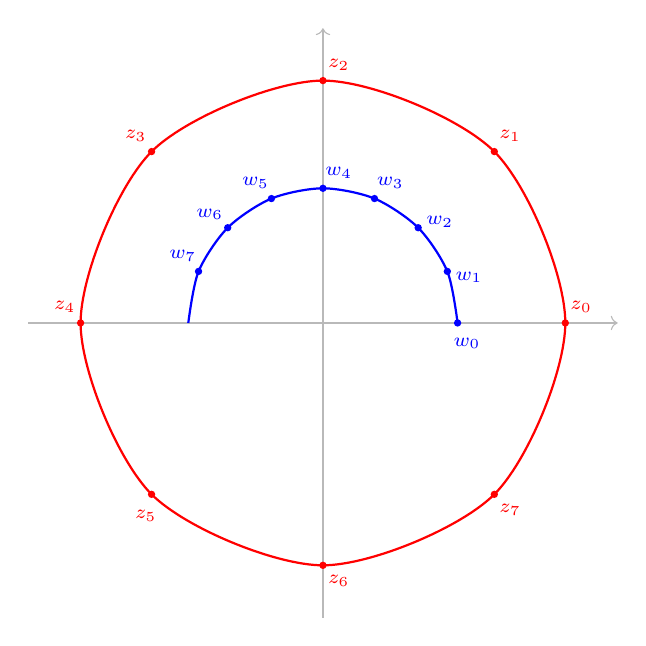
\begin{tikzpicture}[scale=0.95]
  \draw[->,gray!55] (-3.94,0) -- (3.94,0);
  \draw[->,gray!55] (0,-3.94) -- (0,3.94);
  \draw[red,thick] plot[smooth cycle] coordinates {(3.240,0.000) (2.291,2.291) (0.000,3.240) (-2.291,2.291) (-3.240,0.000) (-2.291,-2.291) (-0.000,-3.240) (2.291,-2.291)};
  \fill[red] (3.240,0.000) circle (1.4pt); \node[red,font=\scriptsize] at (3.452,0.212) {$z_{0}$};
  \fill[red] (2.291,2.291) circle (1.4pt); \node[red,font=\scriptsize] at (2.503,2.503) {$z_{1}$};
  \fill[red] (0.000,3.240) circle (1.4pt); \node[red,font=\scriptsize] at (0.212,3.452) {$z_{2}$};
  \fill[red] (-2.291,2.291) circle (1.4pt); \node[red,font=\scriptsize] at (-2.503,2.503) {$z_{3}$};
  \fill[red] (-3.240,0.000) circle (1.4pt); \node[red,font=\scriptsize] at (-3.452,0.212) {$z_{4}$};
  \fill[red] (-2.291,-2.291) circle (1.4pt); \node[red,font=\scriptsize] at (-2.369,-2.581) {$z_{5}$};
  \fill[red] (-0.000,-3.240) circle (1.4pt); \node[red,font=\scriptsize] at (0.212,-3.452) {$z_{6}$};
  \fill[red] (2.291,-2.291) circle (1.4pt); \node[red,font=\scriptsize] at (2.503,-2.503) {$z_{7}$};
  \draw[blue,thick] plot[smooth] coordinates {(1.800,0.000) (1.663,0.689) (1.273,1.273) (0.689,1.663) (0.000,1.800) (-0.689,1.663) (-1.273,1.273) (-1.663,0.689) (-1.800,-0.000)};
  \fill[blue] (1.800,0.000) circle (1.4pt); \node[blue,font=\scriptsize] at (1.927,-0.272) {$w_{0}$};
  \fill[blue] (1.663,0.689) circle (1.4pt); \node[blue,font=\scriptsize] at (1.953,0.611) {$w_{1}$};
  \fill[blue] (1.273,1.273) circle (1.4pt); \node[blue,font=\scriptsize] at (1.563,1.350) {$w_{2}$};
  \fill[blue] (0.689,1.663) circle (1.4pt); \node[blue,font=\scriptsize] at (0.901,1.875) {$w_{3}$};
  \fill[blue] (0.000,1.800) circle (1.4pt); \node[blue,font=\scriptsize] at (0.212,2.012) {$w_{4}$};
  \fill[blue] (-0.689,1.663) circle (1.4pt); \node[blue,font=\scriptsize] at (-0.901,1.875) {$w_{5}$};
  \fill[blue] (-1.273,1.273) circle (1.4pt); \node[blue,font=\scriptsize] at (-1.512,1.453) {$w_{6}$};
  \fill[blue] (-1.663,0.689) circle (1.4pt); \node[blue,font=\scriptsize] at (-1.875,0.901) {$w_{7}$};
\end{tikzpicture}\end{document}
